\chapter{Abordagem Proposta}\label{sec:abordagemproposta}
Neste capítulo é descrita a abordagem proposta para reconhecer emoções por meio da expressão facial e está dividido da seguinte forma. A Seção \ref{sec:monit} detalha o monitoramento do indivíduo. A Seção \ref{sec:detect} descreve um módulo de detecção de face e recorte. A Seção \ref{sec:preproc} aborda as operações de pré-processamento aplicadas na imagem. Na Seção \ref{sec:redeneu} é apresentada a atribuição da rede neural de convolução e por fim um resumo do capítulo na Seção \ref{sec:considfi}.  

\section{Monitoramento do Indivíduo}\label{sec:monit}
Um dispositivo que possui uma câmera fotográfica periodicamente está fotografando o indivíduo. Por exemplo, em um ambiente educacional um \textit{tablet} ou \textit{notebook}, que executa uma plataforma educacional, pode estar monitorando o estudante por meio da câmera frontal ou \textit{webcam}. Este cenário configura um ambiente favorecedor para o monitoramento, pois a câmera frontal ou \textit{webcam} sempre estão capturando as reações do estudante com ângulo frontal. Em um outro exemplo, destacamos uma aplicação para deficientes visuais onde uma câmera apropriada para \textit{wearables} pode estar anexada a roupa do usuário na região peitoral, com intuito de monitorar as reações das pessoas ao redor. Entretanto, este cenário, ao contrário do anterior, possui maiores desafios do ponto de vista de coleta de dados, pois o usuário que está com a câmera pode movimentar-se capturando imagens tremidas, desfocadas e borradas, além de faces com ângulos variáveis. Tais problemas, entretanto, podem ser tratados por equipamentos de qualidade e, portanto, estão fora do escopo deste trabalho. A Figura \ref{fig:arquitetura2} ilustra o fluxo da solução proposta. Portanto, enquanto o monitoramento está ocorrendo, as imagens são enviadas para um repositório de entrada de dados.

\section{Detecção de Face e Recorte}\label{sec:detect}
Este procedimento consiste na detecção de todas as faces de uma imagem por meio do algoritmo Viola Jones (veja Seção \ref{sec:detecfacialviola}). Primeiramente, uma imagem é consumida do repositório de entrada de dados. A detecção consiste na geração de um conjunto de coordenadas que possibilita o desenho de um retângulo indicando a localização da face. Vale ressaltar que esta atividade possui complexidade moderada, pois uma imagem oriunda de cenários reais contém vários objetos com diferentes geometrias, inclusive podendo assemelhar-se a uma face ocasionando a geração de falsos positivos. Logo após a detecção de face, é realizada o recorte da mesma indicada pelo conjunto de coordenadas definidas pela etapa anterior. Tal atividade é valorosa para exclusão do \textit{background}. Desta forma, somente a face recortada é enviada para a fase seguinte, reduzindo a complexidade do problema, pois não há necessidade do classificador aprender a separar o \textit{background} da face. Posteriormente ao recorte da face, a imagem original, que deve estar com uma face recortada, é mantida para nova averiguação de recorte de face. Caso exista outras faces na imagem, este processo é repetido até não existir mais faces para recortar. Obviamente caso seja enviada uma imagem para a etapa de detecção e recorte que não contém uma face (e.g. imagem de um avião) o processo é automaticamente encerrado, pois se não há uma face para detectar, logo não há uma expressão facial emocional para reconhecer. 

\section{Pré-Processamento}\label{sec:preproc}
Uma face recortada é recebida pelo módulo de Pré-processamento. Nesta etapa, operações de pré-processamento são aplicadas com a finalidade de enaltecer as características próprias de cada expressão facial, com intuito de preparar a imagem para a classificação, facilitando a diferenciação das emoções. A Figura \ref{fig:preprocessingfluxo} mostra o fluxo desta etapa. Adicionalmente, uma função de redimensionamento é chamada para transformar a imagem em uma escala de 60x60 \textit{pixels}. Neste trabalho, consideramos que a imagem é colorida, portanto a mesma possui 3 canais denominados RGB (do inglês: Red, Green e Blue), sendo que a imagem resultante possui 10.800 características que pode ser calculada por \textit{Qtd_Caracteristica = N_Pixels_X * N_Pixels_Y * N_Canais}. 
%Após o redimensionamento, é realizado a normalização da imagem dividindo cada \textit{pixel} por 255, isto é, o valor máximo que um \textit{pixel} pode possuir, ocorrendo a normalização dos valores dos \textit{pixels} para o intervalo de 0 a 1. 

A meta principal desta proposta consiste em classificar emoções em qualquer ambiente. Obviamente que a variação do ambiente acarreta em diferentes níveis de intensidade da luz, ocorrendo a perda de características importantes da face que diferenciam as emoções, seja por excesso ou ausência de luz. Vale destacar que esta proposta é baseada principalmente em redes neurais de convolução que originalmente possui vários filtros de pré-processamento. Entretanto, a literatura tem mostrado que filtros clássicos aplicados antes da inserção de uma imagem em redes neurais tem sido eficazes na eliminação de ruídos, principalmente aqueles relacionados a iluminação e brilho \citep{art2,art4,art6}. Portanto, as técnicas de normalização de brilho e iluminação são parte da etapa de pré-processamento, agregando valor para a solução minimizando a sensibilidade relacionada com a variação da luz do ambiente. Assim, a imagem normalizada por filtros de correção de iluminação ressaltará melhor os traços faciais, além da imagem transformada estar com maior nitidez para a continuação do \textit{workflow}.

Este trabalho também foca em minimizar os efeitos negativos de rotações da face e variação da pose para treinamento e classificação. Graus elevados de rotações e poses dificultam a classificação e minimizam o aprendizado, caso a base de treino tenha muita imagem com face rotacionada. Por isso, no pré-processamento é feito o alinhamento da face. Este alinhamento é por meio da localização de três pontos: o canto do olho direito, o canto do olho esquerdo e um ponto central do nariz. Desta forma, esses três pontos formam um triângulo, sendo possível rotacionar a imagem até que não haja uma inclinação na linha dos olhos orientada pelo triângulo. A Figura \ref{fig:face_alinhada} ilustra o exemplo de uma face não alinhada e após o alinhamento. Por fim, nesta etapa, é realizado a normalização da imagem dividindo cada \textit{pixel} por 255, isto é, o valor máximo que um \textit{pixel} pode possuir. Resultando na normalização dos valores dos \textit{pixels} entre o intervalo de 0 a 1. 

\begin{figure}
\centering
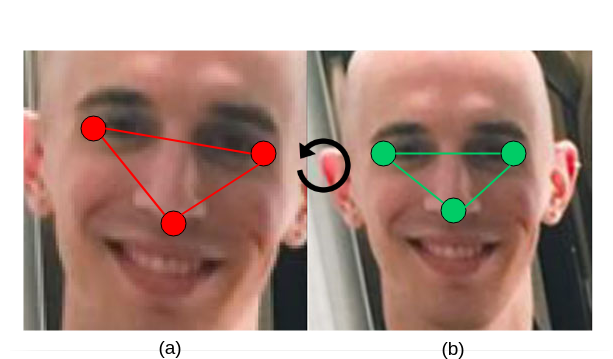
\includegraphics[scale=0.46]{figuras/face_alinhada.png}
\caption{Algoritmo de Alinhamento da Face: (a) Imagem Original; (b) Face Alinhada. }
\label{fig:face_alinhada}
\end{figure}

\begin{figure}
\centering
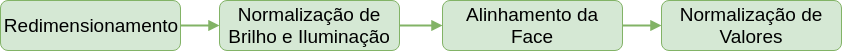
\includegraphics[scale=0.5]{figuras/PreProcessamentoMestrado.png}
\caption{Pré-Processamento fluxo}
\label{fig:preprocessingfluxo}
\end{figure}



\section{Rede Neural de Convolução}\label{sec:redeneu}
A rede neural de convolução é a parte central e com importante contribuição nesta abordagem. Por meio dela, durante o treinamento, as imagens são processadas a fim de aprender os contornos, padrões, formas e características relevantes para a classificação. Além disso, funções são aplicadas para redução de dimensionalidade, extração de características e normalização, ocasionando que a rede não seja sensível a rotações, posições e escala da imagem. Tais aptidões são requisitos para um classificador de imagens ser usado em cenários reais. Apesar de a rede neural ter embutida normalizações e rotações internas, vale a pena realizar as operações da Seção \ref{sec:preproc}, pois são técnicas selecionadas especialmente para o problema de faces, e além disso, a comunidade científica tem descoberto que combinar o processamento interno da rede neural de convolução com outros processamentos externos alcançam os melhores resultados \citep{art2,art4,art6}. Vale ressaltar que um desempenho satisfatório da rede neural de convolução, assim como de qualquer algoritmo supervisionado de aprendizagem de máquina, está estritamente relacionado ao processo de treinamento e validação do modelo.    

\subsection{Treinamento}
O treinamento da rede neural de convolução é parte fundamental para o classificador de emoção funcionar bem. Nesta etapa, é buscado tanto a generalização satisfatória quanto a aquisição do aprendizado suficiente para funcionar em variados ambientes. Para isso, neste trabalho, o treinamento é apoiada pela técnica de aumento de dados com intuito de maximizar a generalização do aprendizado durante o treinamento. O aumento de dados consiste na multiplicação das imagens em tempo dinâmico modificando levemente a imagem e seu contexto, realizando alterações nas imagens aplicando \textit{crop}, rotações, perspectiva, \textit{shear}, diferentes níveis de contraste e dentre outros. Com o propósito de estimular maiores taxas de aprendizado e generalização, pois, assim, a rede neural observa a região de interesse que são as expressões faciais emocionais em diferentes cenários, sendo assim, gerando modelos capazes de classificar emoções em contextos variados. A Figura \ref{fig:aumentoDados} ilustra alguns exemplos da técnica de aumento de dados.

\begin{figure}
\centering
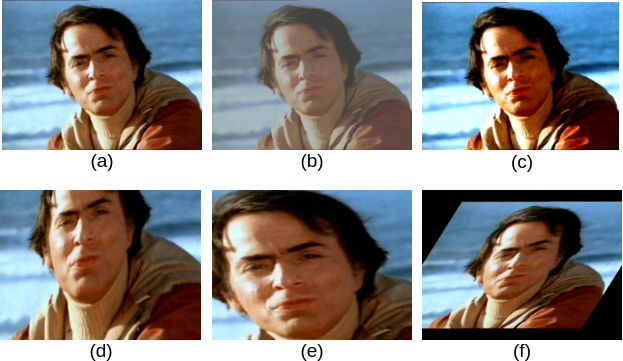
\includegraphics[scale=0.46]{figuras/augmentation.png}
\caption{Exemplos da técnica de aumento de dados: (a) Imagem Original; (b) Redução de Contraste; (c) Aumento de Contraste; (d) Perspectiva; (e) \textit{Crop}; (f) \textit{Shear}. }
\label{fig:aumentoDados}
\end{figure}


\subsection{Extração de Características e Classificação}
Em problemas de classificação de imagem, uma etapa fundamental é a extração de caraterísticas, sendo responsável por retirar de uma entrada de dados as principais informações para enviar a um classificador e, assim, determinar a classe. Na rede neural de convolução, a extração de característica é um procedimento que procura identificar as zonas da imagem que são mais relevantes para a separação do problema, isto é, classificar uma expressão facial (\textit{e.g} o sorriso humano é uma característica indicadora para a emoção felicidade). Este processo funciona com as camadas de convolução da rede operando sobre a imagem retirando as informações relevantes e com a camada de \textit{pooling} aplicando a redução de dimensionalidade. Algumas camadas de convolução tornam-se especialistas na extração dos padrões verticais, outras nos horizontais, em um padrão geométrico especifíco, até que seja gerado um conjunto de características para enviar a um classificador.

%\textit{softmax} classificar estimando a probabilidade para cada emoção.
O classificador recebe as características extraídas, e este fica localizado na última camada da rede neural de convolução. O conjunto extraído é um vetor de uma dimensão que possui uma quantidade de elementos bastante inferior a imagem original. Seu conteúdo consiste no conjunto de informações representativas para diferenciação das emoções que a rede neural aprendeu a extrair no treinamento. Então, o classificador é treinado para separar as emoções. Neste trabalho, o classificador adotado (\textit{softmax}) possui a característica de estimar a probabilidade para cada emoção: neutralidade, raiva, felicidade, tristeza, desprezo, medo e surpresa. E essa estimativa é distribuída entre as classes (\textit{e.g} neutralidade: 0.95, felicidade: 0.25 e surpresa:0.25), possuindo a propridade em que o somatório das probabilidades é igual a 1, e a emoção eleita é a que tem maior probabilidade, nesse caso, a neutralidade com 0.95. A escolha do \textit{softmax} é devido ao mesmo fazer parte da configuração padrão das arquiteturas testadas. Em nossa abordagem, após a classificação de uma imagem, as estimativas de probabilidades geradas são salvas em um repositório de saída de dados. É importante destacar que em uma imagem com mútiplas faces são classificadas uma face por vez, pois é mais simples reconhecer a emoção de uma única face do que em todas ao mesmo tempo.   

%contornos, bordas, linhas, horinzontais, verticais
%Produto de probabilidades Naive Bayes

\begin{figure}
\centering
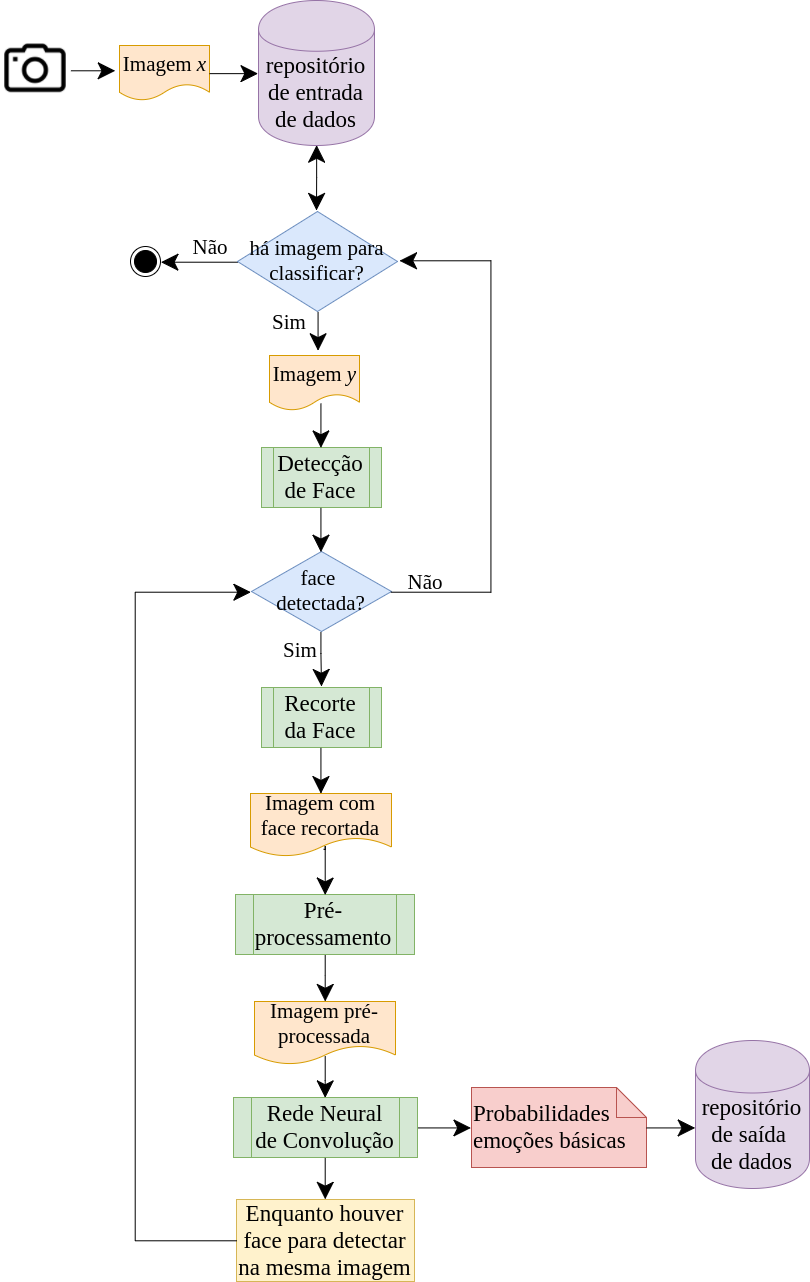
\includegraphics[scale=0.45]{figuras/arquitetura.png}
\caption{Solução Proposta}
\label{fig:arquitetura2}
\end{figure}

     

\section{Resumo}\label{sec:considfi}
%imagens gerais
%LUTE LUTE LUTE LUTE GO FIGHT GO FIGHT YOU CAN ONLY DEPENDS YOU SON OF BEATCH
Neste capítulo foi descrito a abordagem proposta. As principais etapas são: detecção e recorte da face, pré-processamento, extração de características e classificação. A detecção de face consiste na utilização do algoritmo Viola-Jones. Esta etapa gera dois benefícios valorosos que reduzem a complexidade do problema: a exclusão do \textit{background} e o recorte individual de cada face. A etapa de pré-processamento é constituída da aplicação de vários filtros e funções de normalizações na imagem para limpeza, eliminação de ruídos e alinhamento da face. A extração de características é feita pela rede neural de convolução em que procura na imagem pré-processada as informações interessantes para a diferenciação da emoção. Por fim, a etapa de classificação, onde o classificador está localizado na última camada da rede neural de convolução e recebe as informações extraídas para estimar a probabilidade para cada emoção, determinadando as emoções da imagem.      